\documentclass{article}
\usepackage{geometry}
\usepackage{graphicx}
\usepackage{setspace}

% Path to graphic images
\graphicspath{ }

% Title
\title{Wifi Connected Chess Boards \\ \large Feasibility Report Part 3}
\author{Nick Kraus, Kyle Jameson, Maurice Wallace, Mark Mauriello}
\date{\today}

% Margins
\geometry{letterpaper, portrait, margin=.75in}

\doublespacing

\begin{document}

\maketitle

%-----------------------
%		Hardware	
%-----------------------

\section*{Hardware}

\subsubsection*{Embedded System}
\indent

Some more hardware tests have been completed on the individual components to make sure that all pieces will be able to work together in a final product. An electromagnet similar to the one that will be used in the final design was tested with a power supply. The electromagnet was able to move the permanent neodymium magnets at a useful distance (the game board will be able to be made reasonably thick so that the reed switches can be embedded underneath and not obstruct the moving gantry and electromagnet). The neodymium magnets were also able to trigger the reed switches at a distance that will make sure the game board is thick enough to provide a sturdy playing surface. We also got a 20 by 4 character LCD display working with the microcontroller. Using simple functions supplied by Cypress in their LCD API we were able to write strings to the display, erase the display, change characters at specific positions and display custom characters on the display.

\indent

The schematic for the final hardware is nearly complete. Schematic symbols have been created for all parts used in the design, which are stored in separate libraries. The final hardware will be powered from an external third party switching supply which will provide a 12 volt supply from a mains ac socket. This 12 volt supply will be the power input for the final hardware. On the circuit board will be three more power supplies. A 3.3 volt and 5 volt supply will be used to power the WiFi module and microcontroller/peripherals, respectively, and a variable 2-12 volt supply will be used to provide adjustable power to the electromagnet. Many of the peripherals will not be directly on the circuit board and will therefore be connected to the circuit board via soldered header wires. These peripherals include the LCD screen, rotary encoder, reed switch array, stepper motor drivers, limit switch, and electromagnet. The Microcontroller and WiFi module operate at different voltages, which will require an external IO voltage of 3.3 volts to be used by the microcontroller for some of its pins. The Microcontroller, WiFi module, and stepper motor drivers all require decoupling capacitors on the power supply traces to ensure they have enough power available during heavy load times; these have been added to make sure that the supply voltages wont drop when current usage increases. Once the final touches have been put on the hardware schematic a design review can be completed, component footprints can be drawn up, and the circuit board can begin to be designed.

\centerline{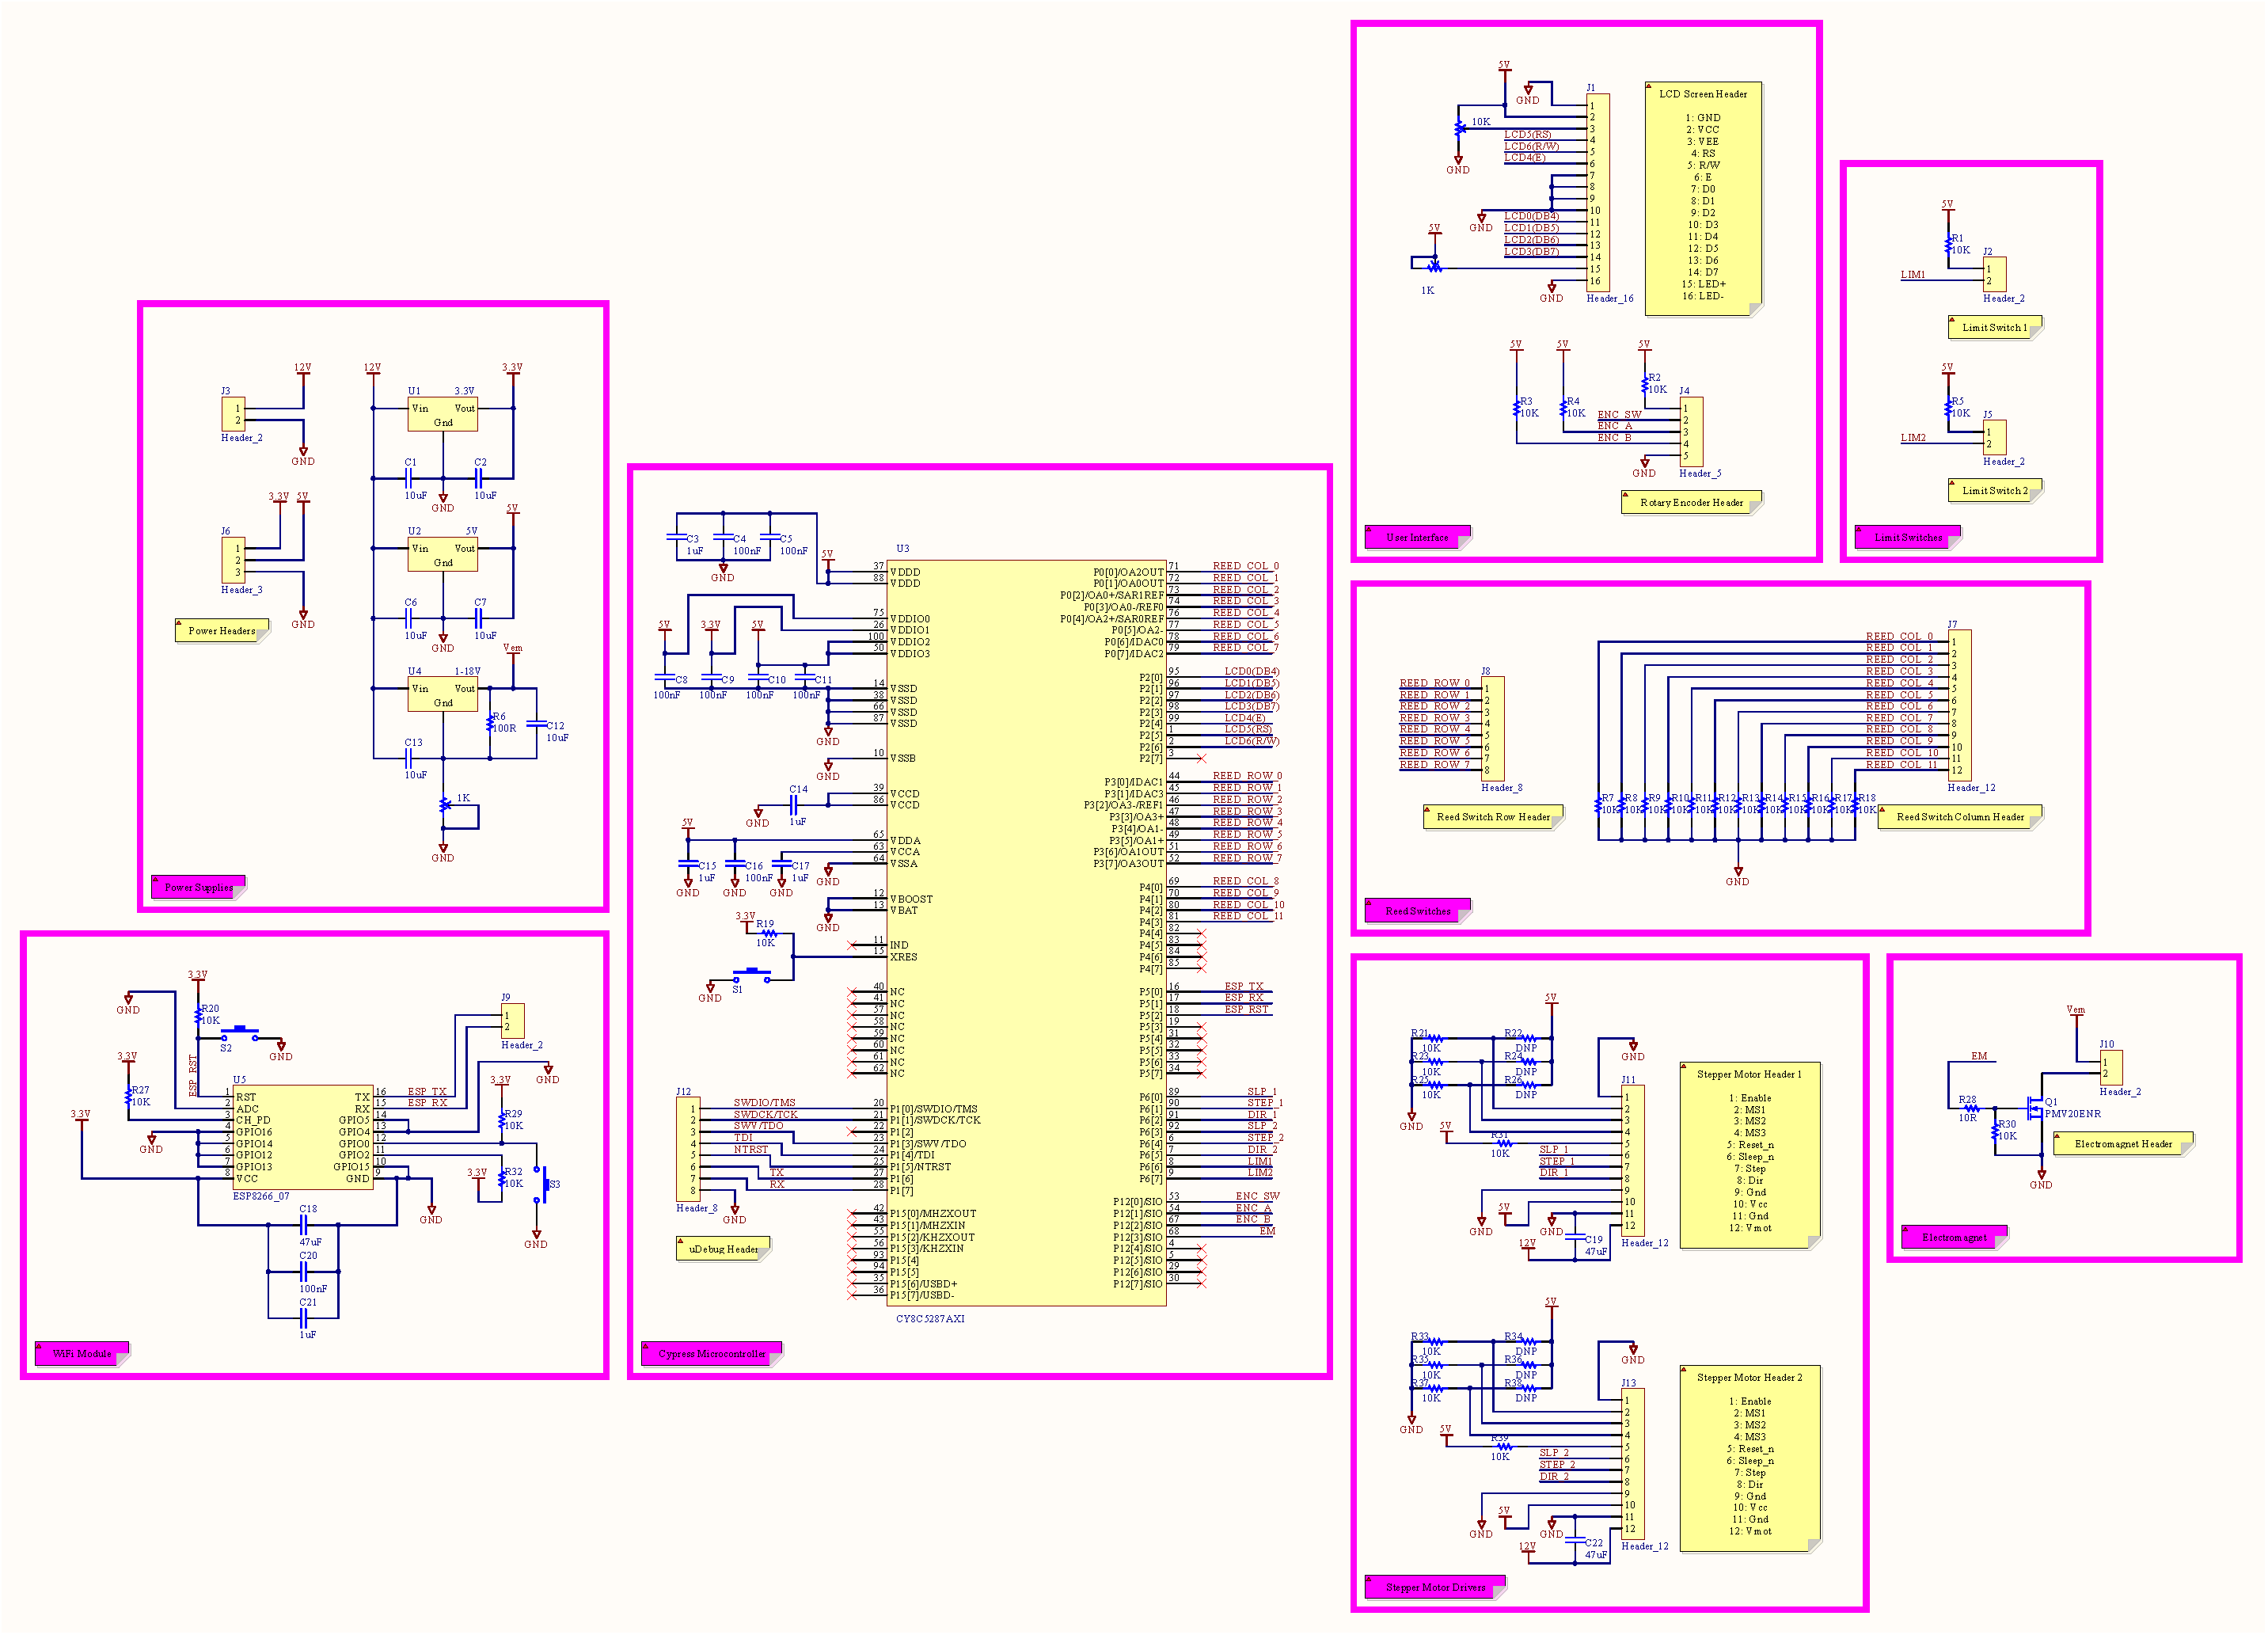
\includegraphics[scale=.5]{Schematic}}

\begin{center}
First revisions of final hardware schematic.
\end{center}

%-----------------------
%		Software	
%-----------------------

\section*{Software}

\subsubsection*{Microcontroller Firmware}
\indent

Regarding the last feasibility report we were able to get the LCD screen to work with the micro controller. We were able to display messages and place them where desired. By using a delay function and clearing the screen it was possible to create timed messages that appeared for a second and then disappeared. Allowing us to rewrite messages on the display. This is the only firmware that was tested on the microcontroller. The other code that was written for the firmware but not tested on the firmware is the algorithms used for keeping track of the chess game. The code here involves initializing the state the game would use, detecting which piece moved in a transition by comparing two states of the board, checking if a move if legal, and a simulation of a game to test the movements by inputting simulated transitions. This software has been tested on the computer to make sure when we implement the mechanical inputs and outputs the code will work properly. Thus code that is dependent on the mechanics for input and output has been simulated for testing purposes. The code that involves controlling the mechanics cannot be implemented and tested until the board has been setup. Although we have been able to test pieces of the mechanics independently before. So we know it is possible to interact with them and receive input and deliver output, which includes the stepper motors and the LCD device. 

\indent

The rest of this paragraph describes what has been completed and done for the code to run the chess game. As of right now the code contains macros for all the pieces and 2 two dimensional arrays for the state and nextState of the game. It also can initialize the start state with all of the pieces in the state character 2d array. When a new state is read, it is stored in nextState which contains 1’s and 0’s as it cannot distinguish the pieces. So there is another function which will compare those states and determine which piece was moved. These transitions are stored and then used in the isLegal function to determine if the transition/move is a valid move. The code for the isLegal function right now has been tested using simulated nextStates or transitions. isLegal as of now can detect when a move is legal if it moves and does nothing else. So the next few parts of isLegal that need to be finished are when a piece is taken, special moves, and moving a piece to the graveyard when a piece is taken. For testing the nextState input has been simulated, transitions have been simulated, the state representing the chess board and it pieces can be printed, and isLegal return values based on transitions can be printed. Thus it is possible to give a list of transitions, check if the moves provided are valid, and change and print the board state without the chess piece graveyard when a transition has been validated.

\centerline{\includegraphics[scale=.5]{IsLegal}}

\begin{center}
Simulation of chess piece move validation.
\end{center}

\subsubsection*{WiFi Module Firmware}
\indent

The Client software that runs the application and controls the mechanical system surrounds the ESP8266 WiFi Module. The WiFi module's original AT-command firmware is overwritten by a custom firmware created in the Arduino IDE. With the IDE, the ESP8266 add-on was installed to allow firmware to be uploaded. This firmware maintains a constant connection with the TCP server, interacting with it by sending bits corresponding to states of the game. The microcontroller will hold responsibility to send the corresponding IP address that the module will connect to. For testing purposes, the client that the module connects to is hard-coded in the code, as well as the chosen port number. Within the Setup() function, the data rate is set, which is 115200 for the module. The program attempts to connect to the network, given an SSID and password. The user is always aware of the status of the connected as the firmware always warns the user if the connection is unsuccessful. The bulk of the operation takes place within the Loop() function which attempts to connect to the server with the hard-coded IP address and port. No further action is taken if the connection fails at this step. The serial monitor provided by the IDE reads input submitted and send this raw data to the TCP server, informing the user of the string that was sent. In the event that the server sends a reply, the module with read it and print it on the serial monitor. Currently, the module is capable of sending and receiving data from the TCP server using the serial monitor in the Arduino IDE. The WiFi module will be improved in the near future to adapt to the game state changes.

\centerline{\includegraphics[scale=.5]{Serial}}

\begin{center}
The serial monitor talking with the WiFi module.
\end{center}

\subsubsection*{Server}
\indent

We are changing the server from an HTTP server back to a TCP server. This will give us more control over what the server and client will send to each other. It will be much easier for us to parse the TCP message than the HTTP message. The simplicity of using TCP will keep our code readable and maintainable. Another advantage is that we can create our own protocol so that the server and client can send and receive messages they both understand. This will require the person writing the server software to work with the person writing the WiFi module firmware and the person writing the microcontroller code to develop a protocol that all three can work with. Some commands that a client needs to send to the server are: picking a side of the board, starting a game, moving a piece, declaring check and checkmate, declaring a draw or stalemate, and others. These can be broken off into their own functions in Python, which the server can run depending on what the WiFi module sent.

\centerline{\includegraphics[scale=.5]{Server}}

\begin{center}
The server responding to a request from the WiFi module.
\end{center}

\end{document}